%----------------------------------------------------%
%                    INTRODUCCION                    %
%----------------------------------------------------%

\pagestyle{fancy}

\chapter{Introducción}
\label{introduccion}

Desde Aristóteles y su libro Segundos Analíticos \footnote{\href{https://docs.google.com/a/datik.es/file/d/0By4kcbi6MzzdUHhVQnUtcTNUdk0/view}{Órganon II de Aristóteles: Segundo Analíticos se encuentra recopilado en él}} hasta Galileo, padre de la ciencia moderna, adalides del conocimiento han proclamado que un método de investigación basado en lo empírico y en la medición, sujeto a los principios específicos de las pruebas de razonamiento es el camino para conocer la verdad.\\

Hoy en día, época en la que los avances tecnológico han posibilitado observar y medir de forma exhaustiva un gran abanico de fenómenos, la ingente cantidad de datos que se genera en el proceso es, a veces, intratable por medio de las tecnologías convencionales, y por ende, es imposible extraer conocimiento. El problema, lejos de atenuarse, se acrecienta con el paso del tiempo, ya que, estudios como el realizado por McKinsey Global Institute estiman que el volumen de datos que se genera crece un 40\% cada año y auguran que entre 2009 y 2020 se verá multiplicado por 44 \cite{nambiartowards}.\\

Por ello, en los últimos años ha irrumpido la necesidad de encontrar tanto metodologías como tecnologías que permitan procesar y extraer el conocimiento que atesora el torrente de información en la cual se encuentra envuelta la sociedad, dando como resultado el nacimiento del Big Data.\\

El mundo empresarial, por su parte, no se ha mantenido al margen de esta gran revolución. Conscientes de los beneficios que les puede reportar en diferentes aspectos como en el análisis de mercado y mejora en la calidad de los servicios, la gran mayoría de las empresas se han interesado en este fenómeno. De un estudio realizado entre los altos ejecutivos de las firmas que lideran el Wall Street se desprende que el 96\% tiene planeadas ciertas iniciativas relacionadas con el Big Data, y el 80\% ya tiene finalizada alguna \cite{bdes:2013}. 

\section{Contexto}
 
Datik Información Inteligente \footnote{\url{http://www.datik.es/}} es una empresa tecnológica perteneciente al Grupo Irizar \footnote{\url{http://www.irizar.com/irizar/}}  que desarrolla soluciones ITS destinadas a la gestión del trasporte, tanto ferroviario como por carretera y movilidad ciudadana.\\

Uno de los productos estrella de la entidad es el denominado iPanel, concentrador de  información que ofrece al operador de transporte servicios de valor añadido en la gestión de la información generada por su flota. El funcionamiento del servicio se puede resumir mediante la Figura \ref{fig:ipanel}:\\

\begin{figure}[h]
	\centering
	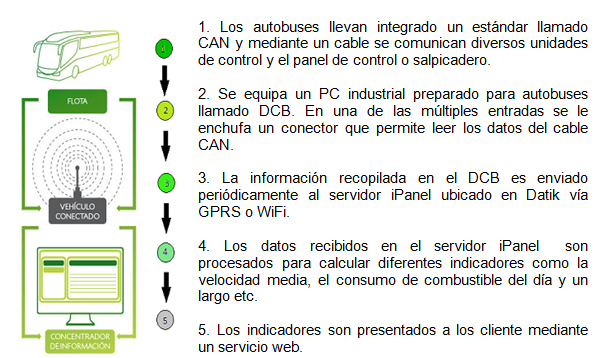
\includegraphics[width=1\textwidth]{Ilustraciones/ipanel_infraesctructure.png}
	\caption{Funcionamiento resumido de iPanel}
	\label{fig:ipanel}
\end{figure}

La incesante integración de nuevos vehículos a iPanel ha generado un crecimiento exponencial en el número de registros almacenados en ciertas tablas de MySQL. Aunque el volumen actual no suponga riesgo alguno para el funcionamiento del servicio, Datik tiene identificados varios escenarios en los que la situación se podría revertir, causando graves problemas en el sistema.\\

El primero de todos, es la corrupción de datos. Este fenómeno sucede debido a un bug, fallo de almacenamiento inesperado, o una caída de MySQL cuando el resultado del checksum de una página es diferente al esperado. Aunque ocurre de forma esporádica, compromete seriamente la información que Datik ofrece a sus clientes mediante la aplicación web.\\ 

Otro de los problemas, intrínseco a depender de una base de datos centralizada, es el operar sobre un único punto de fallo. Debido a que la mayoría de procesos confluyen en ella, el bloqueo o la caída causada por un servicio puede acarrear la de otros, a priori, totalmente independientes. Para solventar el problema Datik ha optado por migrar su infraestructura a una basada en Microservicios \cite{newman2015building}, logrando de esa manera, el aislamiento total de los componentes que conforman su ecosistema.\\ 

El último problema, es el referente al proceso denominado Cálculo de Indicadores, el cual se ejecuta una vez al día para realizar operaciones aritméticas sobre diversas tablas y después, agrupar los resultados en base a diferentes criterios. Siendo dichas tablas las que mayor crecimiento experimentan, el aumento del volumen de las mismas incrementa de forma desorbitada el tiempo necesario para finalizar el cálculo, pudiendo, en un futuro, llegar a tardar mas de 24 horas y cancelar los indicadores que ofrecen información del último día.\\

El objetivo del presente proyecto es proponer soluciones a los problemas planteados en este apartado, haciendo especial hincapié en el proceso Cálculo de Indicadores, ya que afecta de forma directa a la información que consumen los clientes de Datik vía iPanel.\\

\section{Propuesta}

La problemática que envuelve al proceso Cálculo de Indicadores tiene origen en el incremento exponencial del número de registros a tratar. No sería descabellado pensar que la solución pasa por aumentar los recursos destinados a la máquina y afinar la configuración de MySQL. No obstante, existe un límite a la hora de escalar verticalmente y cuanto más se afine dicha configuración, la mejora será menos acentuada. Mientras, el volumen de los datos seguirá aumentando de forma inexorable, volviendo, tarde o temprano, a tener que lidiar con los mismos problemas.\\

Siendo imposible reconducir la situación mediante el uso de la tecnología tradicional, en el presente proyecto se propone realizar un cambio de paradigma en la forma y modo que se trata la información relacionada con el proceso cálculo de indicadores.



* Diseccionar el problema: almacenamiento y procesamiento
* diseccionando el problema / dos vertientes
datos no relacionales, nosql parece buena alternativa

Analizando el escenario presentado, 

Para solventar los problemas que Datik prevé, se propone implantar las tecnologías Apache Cassandra y Apache Spark en la empresa y migrar tanto las tablas como los procesos que son parte en el cálculo de los indicadores.\\


Apache Cassandra es una base de datos distribuida no-sql. Gracias a naturaleza distribuida ayuda a resolver, 

Funcionalidades nuevas que trabajan con videos etc




Diseñar un plan de migración que defina aspectos tales como: 

\begin{itemize}
	\item Listado de las tablas MySQL que deben ser migradas a Cassandra priorizando las que más rápido crecen y mayor número de consultas intensivas reciben. Por ejemplo, las tablas que contienen la información para el calculo de los indicadores.
	\item Listado tablas "frontera"
	\item Ver por cada ejercicio su estado de realización: quiénes lo han terminado, quiénes tienen duda y quiénes no han respondido nada.
	\item Editar cualquier detalle de un ejercicio en cualquier momento.
	\item Valorar la realización de un ejercicio a un alumno concreto.
\end{itemize}

el traspaso de las tablas MySQL que mayor velocidad crecen  y mayor número de consultas pesadas reciban a estas nuevas tecnologías. empezando por las que tienen estrecha realción con el calculo de indicadores, ya que, como se ha indicado con anterioridad, es  

Por su parte, Apache Cassandra

Por Apache Spark por otra,

Debido a la falta de datos se ha utilizado un dataset publico para emular las condiciones de futuro con las que se va a encontrar datik

\section{Organización del documento}

En esta memoria se ha documentado  el desarrollo de la herramienta \textbf{\textit{exerClick}}, dentro del Trabajo de Fin de Grado (TFG) del autor. En el documento se describe la propuesta, la planificación y gestión que esta lleva consigo, la implementación llevada a cabo y las conclusiones finales.\\

En este primer capítulo se ha introducido el problema a resolver y se ha explicado la propuesta presentada en este proyecto.\\

En el capítulo 2 se presenta el Documento de Objetivos de Proyecto (DOP). Este recoge el alcance y las fases y tareas del proyecto, el análisis de riesgos y el análisis de factibilidad.\\

Una vez en el capítulo 3 se explica la gestión llevada a cabo durante el proyecto. Se presentan las metodologías utilizadas: Metodologías Ágiles e InterMod (adaptada a las necesidades de este proyecto). A continuación se detallan cada una de las iteraciones llevadas a cabo (como parte de la metodología InterMod): duración, objetivos y tareas realizadas. Al final del capítulo se muestra la documentación asociada a las iteraciones y los objetivos, además del seguimiento de tiempo realizado.\\

A continuación, en el capítulo 4 se detalla el análisis de requisitos. Primero se detallan los requisitos no-funcionales y luego los funcionales (prototipos en papel llevados a cabo durante las primeras iteraciones que dan una visión global del proyecto).\\

En el capítulo 5 se explica el diseño e implementación llevados a cabo. Se comienza mostrando la estructura de documentos del proyecto, luego el diseño realizado en base al análisis de requisitos del capítulo 4 y finalmente una visión general de la implementación de la lógica de negocio.\\

Para finalizar, en el capítulo 6 se presentan las conclusiones, líneas futuras para el proyecto y las lecciones aprendidas.\\

Fuera de la estructura general de la memoria, tenemos la bibliografia y los apéndices. En estos últimos tenemos las actas de reuniones, las actas de pruebas y la vista de relaciones de la base de datos (de la parte utilizada o creada específicamente para el proyecto).\\